\section{Py Serial}

	\subsection{Python}
	Python adalah bahasa pemrograman yang dibuat oleh Guido van Rossum dan populer sebagai bahasa pemrograman scripting dan Web. Mengacu pada ide wikipedia, Python adalah bahasa pemrograman interpretatif multiguna dengan filosofi desain yang berfokus pada keterbacaan kode. 
	Berasal dari 1991, Python adalah bahasa pemrograman yang relatif baru. Dari awal, Python dianggap sebagai pengisi celah, cara untuk menulis skrip yang mengotomatiskan hal-hal membosankan seperti salah satu buku populer tentang belajar Python meletakkannya atau dengan cepat prototipe aplikasi yang akan diimplementasikan dalam satu atau lebih bahasa lain .
	Namun, selama beberapa tahun terakhir, Python telah muncul sebagai warga kelas satu dalam pengembangan perangkat lunak modern, manajemen infrastruktur, dan analisis data. Ini bukan lagi bahasa utilitas ruang belakang, tetapi kekuatan utama dalam pengembangan aplikasi web dan manajemen sistem dan pendorong utama di balik ledakan dalam analitik data besar dan kecerdasan mesin
	Python dikenal sebagai bahasa pemrograman yang menggabungkan nilai nilai kapabilitas, kemampuan, dengan sintaks kode yang sangat begitu jelas, dan dilengkapi dengan fungsi penyimpanan standar yang menjadikannya komprehensif dan komprehensif. 
	Python memiliki salah satu fitur yang sangat unik yaitu sebagai bahasa pemrograman dinamis yaitu yang datang dengan manajemen memori otomatis. Seperti bahasa 
	Python berjalan di setiap sistem operasi utama dan platform, dan yang paling kecil juga. Banyak pustaka utama dan layanan bertenaga API memiliki binding atau pembungkus Python, memungkinkan Python untuk secara bebas berinteraksi dengan layanan tersebut atau menggunakan perpustakaan tersebut secara langsung. Python mungkin bukan bahasa tercepat, tetapi apa yang kurang dalam kecepatan, itu membuat dalam fleksibilitas.
	Python bukan bahasa mainan. Meskipun scripting dan otomatisasi menutupi sebagian besar kasus penggunaan Python lebih lanjut di bawah, Python juga digunakan untuk membangun perangkat lunak berkualitas profesional yang kuat, baik sebagai aplikasi yang berdiri sendiri maupun sebagai layanan web.
	Python dapat digunakan untuk berbagai tujuan pembuatan perangkat lunak atau pun pengembangan perangkat lunak dan dapat dijalankan di berbagai platform sistem operasi. Python adalah salah satu contoh bahasa tingkat tinggi. 
	Contoh lain dari bahasa high-rise adalah pascal, c ++, perl, java, dan seterusnya. Sedangkan bahasa tingkat rendah adalah bahasa mesin atau bahasa assembly. 
	Secara sederhana. komputer hanya dapat menjalankan program yang ditulis dalam bahasa mesin. Karena itu. jika sebuah program ditulis dalam bahasa tinght yang tinggi. maka program tersebut harus diolah terlebih dahulu sebelum dapat dijalanlon di komputer. 
	Ini adalah salah satu kekurangan bahasa tingkat tinggi yang membutuhkan waktu untuk memproses suatu program sebelum dijalankan. Namun, bahasa tingkat tinggi memiliki banyak kelebihan. Bahasa tinglrat yang tinggi mudah dipelajari. mudah ditulis. mudah dibaca. dan tentu saja mudah menemukan kesalahan. Bahasa tingkat tinggi juga mudah dibawa untuk dicocokkan dengan mesin yang menjalankannya. 
	Ini berbeda dari bahasa mesin yang hanya bisa digunakan untuk mesin. Dengan kelebihan ini. kemudian banyak aplikasi yang ditulis menggunakan bahasa tinflrat yang tinggi. 
	Proses konversi dari bahasa tingkat tinggi ke tingkat rendah dalam bahasa pemrograman adalah tipe. Itu adalah penerjemah dan kompilator. penerjemah membaca program bahasa tingkat tinggi kemudian menjalankan program. 
	Ini berarti interpreter melakukan apa yang dikatakan dalam program. Bisa dibilang. interpreter dibaca per baris dan kemudian telusuri.
	Keberhasilan Python berkisar pada beberapa keuntungan yang disediakan untuk pemula dan para ahli:
	
	\subsection{Kelebihan}
		\begin{itemize}
			\item Python mudah dipelajari.
			\item Dapat lebih cepat dalam pembuatan sistem aplikasi.
			\item Programnya lebih fleksible, singkat, dan sederhana.
			\item Dapat lebih mudah hindari pencatatan kode.
			\item Sintaks Python dirancang agar mudah dibaca dan lugas.
			\item Dapat lebih cepat dalam membuat sistem aplikasi dengan menggunakan objek yang telah ada.
			\item Mempunyai dukungan pemrograman dengan skala yang besar.
			\item Ekstensinya lebih sederhana juga berkas binernya kecil.
			\item Dapat memodifikasi atau merubah aplikasi tanpa menghentikannya.
			\item Kecepatan dalam mengeksekusi bertambah juga melindungi kode sumber.
		\end{itemize}
		
	\subsection{Kekurangan}
		\begin{itemize}
			\item Python tidak efisien sebagai sebuah statis, berbeda dengan bahasa C yang dapat mempunyai penugasan yang lebih luas dari python.
			\item Python adalah sebuah interpreter, jadi tidak begitu baik dalam pengantar komponen performa kritis.
			\item Tidak bisa menjadi dasar bahasa pemrograman implementasi di beberapa komponen.
			\item Tidak memberikan keefensiensian yang menyeluruh.
		\end{itemize}
	
	\subsection{Kegunaan Python}		
	Kasus penggunaan paling dasar untuk Python adalah sebagai bahasa scripting dan otomasi. Python tidak hanya pengganti skrip shell atau file batch, 
	tetapi juga digunakan untuk mengotomatiskan interaksi dengan browser web atau aplikasi GUI atau penyediaan dan konfigurasi sistem di alat seperti 
	Ansible dan Salt. Tetapi scripting dan otomatisasi hanya mewakili puncak gunung es dengan Python.
		\begin{itemize}
			\item Python digunakan untuk pemrograman aplikasi umum.
			\item Python digunakan untuk ilmu data dan pembelajaran mesin.
			\item Python digunakan untuk layanan web dan API RESTful.
			\item Python digunakan untuk metaprogramming.
			\item Python digunakan untuk glue code
		\end{itemize}
	
	\subsection{Proyek menggunakan PySerial}
		\begin{itemize}
			\item BitPim : aplikasi crossplatform untuk melihat dan memanipulasi data pada ponsel CDMA dari LG, Samsung, Sanyo dan produsen lainnya.
			\item RFIDIOt : pustaka python open source untuk menjelajahi perangkat RFID (lihat juga \"e-paspor RFID yang memungkinkan bukti kode konsep dirilis 
			(RFIDIOt)\" dan \"Kode menyoroti risiko e-passport eavesdropping\")
			\item t616hack : distribusi yang menyediakan akses ke kontak, buku telepon dan pesan di Sony Ericsson T610 / T616 dan telepon seluler yang kompatibel
			\item jaraco.nxt : paket yang menerapkan komunikasi API tingkat rendah dengan kit robot LEGO Mindstorms NXT.
			\item Twisted : Menggunakan pySerial untuk menyediakan transportasi port serial asynchronous yang dapat digunakan seperti transportasi stream-oriented 
			lainnya (misalnya TCP, SSL).
		\end{itemize}
	
	\subsection{Komunikasi Serial}
		Langkah - langkah untuk melakuan komunikasi serial adalah sebagai berikut :
		
		\begin{enumerate}
			\item Open Phyton Shell
			
				\begin{figure}[ht]
			\centerline{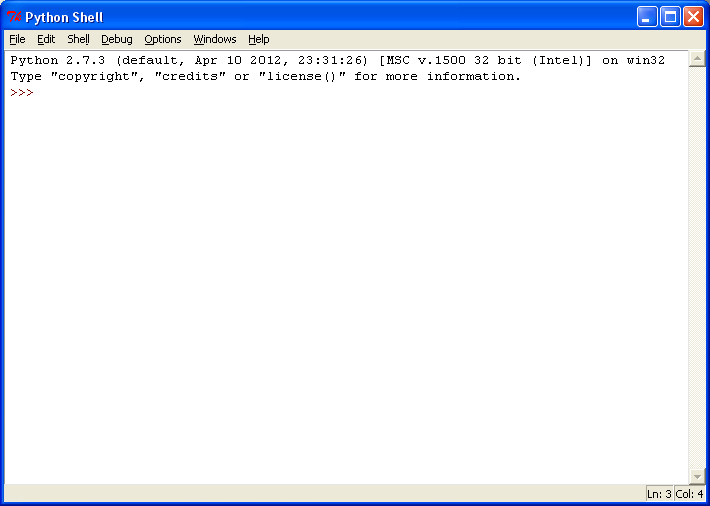
\includegraphics[width=0.5\textwidth]{figures/pyshell.png}}
			\caption{Python Shell}
			\label{pyshell}
			\end{figure}
			
			\item Buat new window seperti atau bisa juga dengan (Ctrl + N), agar muncul window baru.
				
				\begin{figure}[ht]
			\centerline{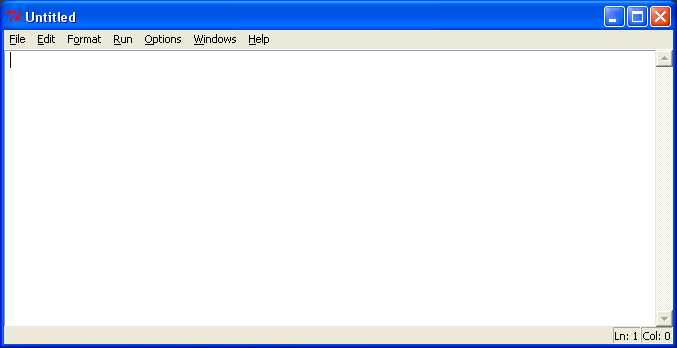
\includegraphics[width=0.5\textwidth]{figures/pyshellnew.png}}
			\caption{New Window}
			\label{pyshellnew}
			\end{figure}
			
			\item Copykan atau ketikkan script ini :
				\begin{verbatim}
					    import serial
						ser = serial.Serial(‘com10’,9600,timeout=1)
						from Tkinter import *
						root=Tk()
						def task():
						a=ser.readline(1)
						print “nilai= ” + a
						root.after(200,task)
						root.after(200,task)
						root.mainloop()
					\end{verbatim}
					
			\item Dibawah ini adalah hasilnya :
			akan muncul window:
			
			\begin{figure}[ht]
			\centerline{
\includegraphics[width=0.5\textwidth]{figures/tkser.png}}
			\caption{TK Window}
			\label{tkser}
			\end{figure}
			
			dan di Python Shell akan muncul :
			
			\begin{figure}[ht]
			\centerline{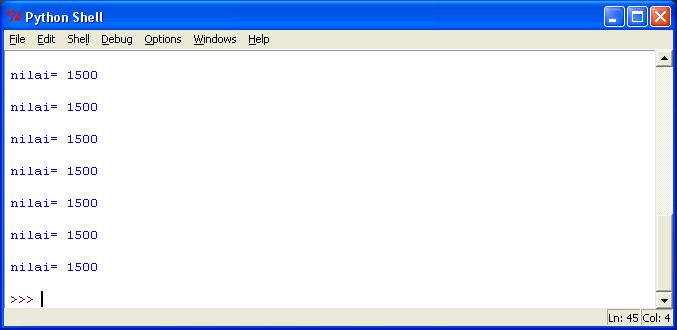
\includegraphics[width=0.5\textwidth]{figures/tkpython.png}}
			\caption{TK Window}
			\label{tkpython}
			\end{figure}
			
		\end{enumerate}
		
		Penjelasannya : 
		\begin{itemize}
			\item import serial
			bagian diatas ini mempunyai fungsi untuk melibatkan module serial sehingga dapat digunakan pada Python.
			
			\item \begin{verbatim} ser = serial.Serial(‘com10’,9600,timeout=1)\end{verbatim}
			Bagian diatas ini berfungsi sebagai pendeklerasian variabel ser sebagai serial port yang propertinya adalah konfigurasi nomer port= COM10, baudrate= 9600, dan timeout=1.
			\item \begin{verbatim} a=ser.readline() \end{verbatim}
			Bagian diatas ini berfungsi untuk membaca data dari serial lalu menampungnya pada variabel a sebagai buffer.
			\item \begin{verbatim} print “nilai= ” + a \end{verbatim} 
			Bagian diatas ini berfungsi untuk tampilkan nilai yang didapat di Python Shell. 
			\item \begin{verbatim} root.after(200,task) \end{verbatim}
			Bagia di atas ini berfungsi untuk melakukan suatu schedule setiap 200 milidetik.
			\item \begin{verbatim} root.after(200,task)	\end{verbatim}
			Bagian diatas ini berfungsi untuk mengulang suatu schedule setiap 200 milidetik.
			\item \begin{verbatim} root.mainloop() \end{verbatim}
			Bagian diatas ini berfungsi untuk melakukan perulangan atau loop.
		\end{itemize}
	
	\cite{nurjanahhack}
	\cite{rossum1995python}
	\cite{chun2001core}
